\section{Što je konvolucija}
Konvolucija je u svojoj srži jednostavna matematička operacija koja je prikladna za obradu signala.
U osnovi, fotografija je vrsta signala, a konvolucija je crna kutija koja pretvara jedan signal, odnosno sliku, u drugi.
Prednost konvolucije je što ne gleda samo jednu vrijednost već i susjedne vrijednosti, pružajući tako dodatan kontekst.

\section{Jezgra konvolucije (\emph{eng. Kernel})}
Jezgra konvolucije, često nazvana \emph{prozor}, je matrica malih, neparnih dimenzija najčešće $3 \times 3$ ili $5 \times 5$.
Primjer jezgre može biti: 
$$
\begin{bmatrix}
	-1 & 0 & -1 \\
	-1 & 8 & -1 \\
	-1 & 0 & -1
\end{bmatrix}
$$
Jezgrom se prelazi preko željene matrice svim retcima i stupcima izvodeći u svakom koraku množenje po članovima (\cite{conv_pres}), primjerice:

\[
\begin{bmatrix}
	4 & 1 & 5\\
	1 & 2 & 6 \\
	9 & 7 & 3
\end{bmatrix}
\times
\begin{bmatrix}
	-1 & 0 & -1 \\
	-1 & 8 & -1 \\
	-1 & 0 & -1
\end{bmatrix}
=
\begin{bmatrix}
	-4 & 0 & -5\\
	-1 & 16 & -6 \\
	-9 & 0 & -3
\end{bmatrix}
\]
Jezgra konvolucije, i sama konvolucija su prikladni za obradu slike iz razloga što računalo sliku i vidi kao dvodimenzionalnu matricu.
Lako je zamislivo, posebice u slučaju crno-bijele slike gdje vrijednosti mogu biti $\in [0, 255]$, gdje je $0$ crna, a $255$ bijela boja.

\subsection{Rubne vrijednosti}
Problem koji se može javiti je kako baratati rubnim vrijednostima za potrebe korištenja u jezgri.
Na primjer, gornji lijevi rub slike nema susjedne vrijednosti gore i lijevo od sebe.

\paragraph{Produljivanje}
u slučaju nedostatka susjedne vrijednosti na njegovo mjesto samo kopira najbližu postojeću vrijednost (Ilustracija \ref{fig:extend_edge}).

\paragraph{Obgrljivanje}
promatra sliku kao da je beskonačna po veličini u obje osi.
U slučaju nedostatka vrijednosti  jednostavno dobiva vrijednost sa suprotne strane.
Također, to je metoda koju sam ja koristio u implementaciji i eksperimentima te pruža dobre rezultate (Ilustracija \ref{fig:wrap_edge}).

\paragraph{Preskakivanje}
uopće ne promatra rubne vrijednosti slike te zaobilazi problem nepostojećih rubnih vrijednosti u potpunosti.
Problem koji se može javiti je da je rezultantna matrica $G$ manja od izvorne matrice $F$.

\begin{figure}
	\caption{Grafički prikaz dva različita načina upravljanja rubnim vrijednostima s označenim rubom slike i trenutnom pozicijom jezgre}
	\begin{subfigure}[t]{0.48\textwidth}
		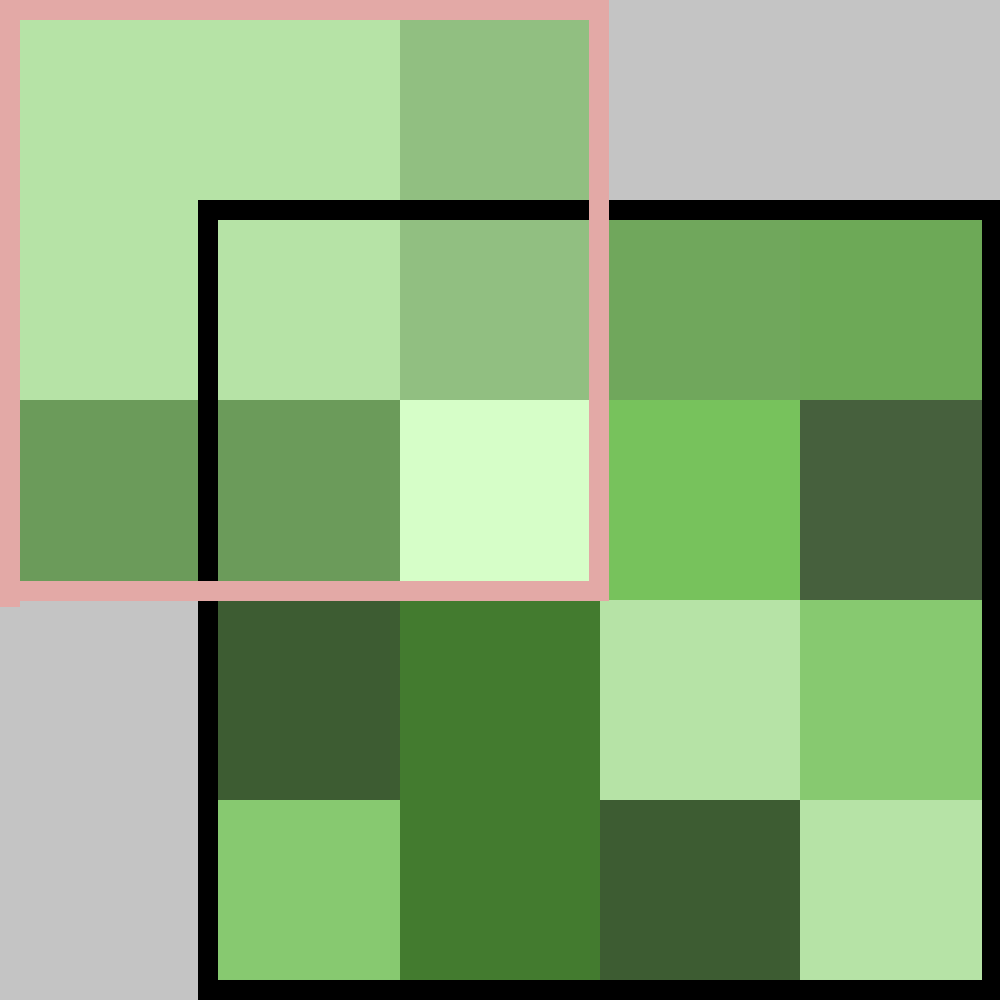
\includegraphics[width=\textwidth]{Illustrations/extend.png}
		\caption{Upravljanje rubom produljivanjem trenutno promatrane jezgre}
		\label{fig:extend_edge}
	\end{subfigure}
	\begin{subfigure}[t]{0.48\textwidth}
		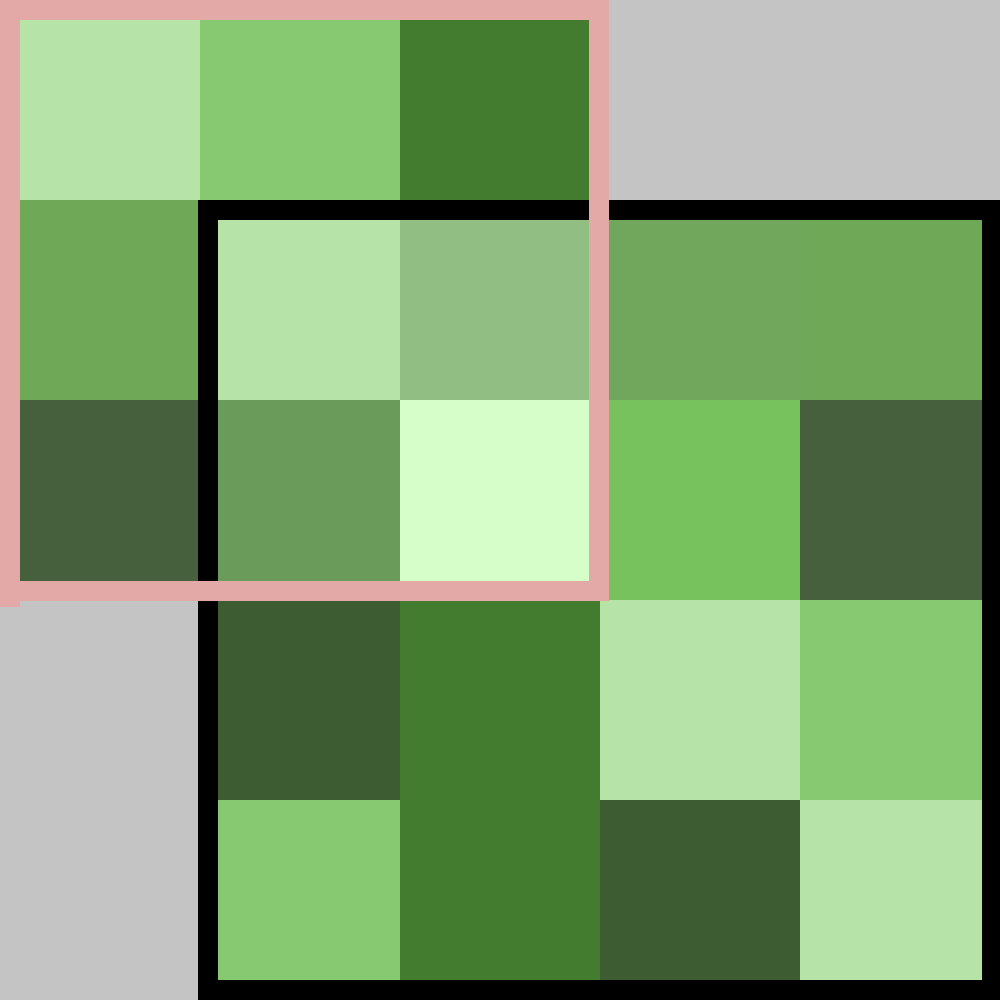
\includegraphics[width=\textwidth]{Illustrations/wrap.png}
		\caption{Upravljanje rubom obgrljivanjem slike}
		\label{fig:wrap_edge}
	\end{subfigure}
\end{figure}

\section{Operacija konvolucije}
Konvolucija se matematički može prikazati kao
$$g(x, y) = \omega \cdot f(x,y) = \sum_{dx=-a}^{a} \sum_{dy=-b}^{b} \omega(dx, dy)\cdot f(x + dx, y + dy)$$
gdje je $g(x,y)$ rezultantna slika, $f(x, y)$ izvorna slika a $\omega$ jezgra (\cite{conv_wiki}).
